\documentclass{beamer}
 
\usepackage[utf8]{inputenc}
\usepackage{lmodern}% http://ctan.org/pkg/lm
\usepackage[demo]{graphicx}
 
 
%Information to be included in the title page:
\title{Survival Analysis of iFixit's Online Question and Answer Forum}
\author{Lisa Oshita}
\institute{Bill and Linda Frost Fund\\
Frost Research Fellow\\
Recipient of the Frost Undergraduate Student Research Award}
\date{2017}
 
 
\begin{document}
 
\frame{\titlepage}

%background information on iFixit
\begin{frame}
\frametitle{iFixit}
  \begin{itemize}
    \item Founded in 2003 by two engineering students here at Cal Poly 
    \item Provides over 30,000 free repair guides
    \item Sells specialized tools/parts needed for repair 
  \end{itemize}
\end{frame}


\begin{frame}
  \begin{figure}
  \centering
    \begin{subfigure}{0.5\textwidth}
        \includegraphics[width=1\linewidth]{question}
    \end{subfigure}
    \begin{subfigure}{0.5\textwidth}
        \includegraphics[width=1\linewidth]{answer}
    \end{subfigure}
  \end{figure}
\end{frame}

%some descriptive statistics of the data + answer times
%Longest answer time: 2159.022 hours (36 days)
%Shortest answer time: 0.008 hours (0.5 minutes) 
\begin{frame}

\frametitle{The Data}
  
  \begin{columns}
      \begin{column}{0.5\textwidth}
          \begin{figure}
            \includegraphics[width = 1.0\textwidth]{answersdist} 
          \end{figure}
      \end{column}
      \begin{column}{0.5\textwidth}
          \begin{figure}
            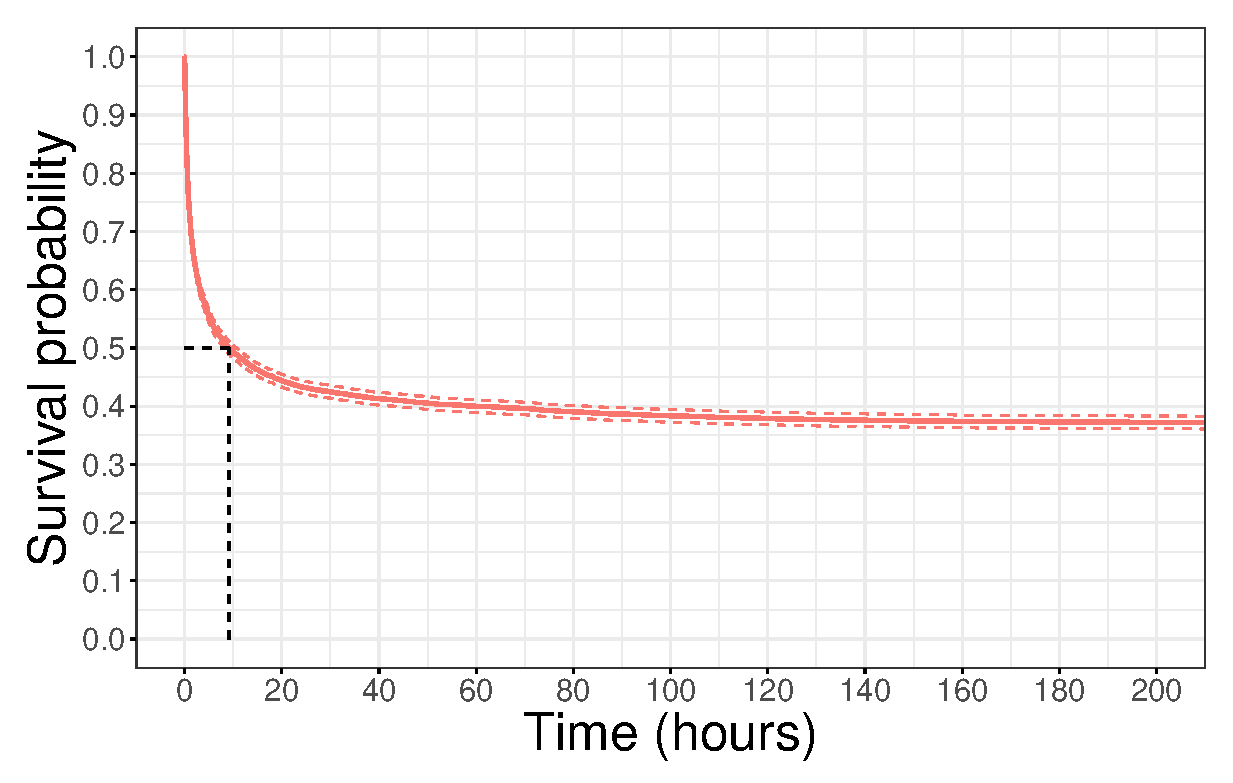
\includegraphics[width = 1.0\textwidth]{kmcurve}
          \end{figure}
      \end{column}
  \end{columns}
  
\bigskip

  \begin{itemize}
      \item 7,760 questions posted between April 8, 2017 to July 7, 2017
      \item 63.8\% recieved an answer by the download date
      \item Median survival time, the time at which 50\% of the questions in the data recieved an answer, is 9.16 hours
  \end{itemize}
  
\end{frame}

% describe how I analyzed the data  
% test data = 6,208 questions, training data = 1,552 questions
\begin{frame}
\frametitle{Methods}
  
  \begin{itemize}
      \item Used text mining and string manipulation techniques to create variables
      \item 5-fold cross validation: 5 training and test data sets 
      \item Assessed performance metrics
      \item Stratified on the time of day the question was posted
      \item Included splines on quantitative variables like the average length of a question's tags
  \end{itemize}
  
\end{frame}

% describe results of fitting model to full data 
\begin{frame}
\frametitle{Results}

  \begin{itemize}
      \item r-square = 0.155
  \bigskip
      \item Interpretations of coefficients:
      \begin{itemize}
          \bigskip
          \item Estimated hazard of receiving an answer is 155\% higher \\ (95\% CI (131.1\%, 182.8\%)) 
          for questions pertaining to Apple products than the hazard for questions about Android and Other Phones,
          controlling for other predictors.
          \bigskip
          \item Estimated hazard of receiving an answer is 31.3\% higher \\ (95\% CI (22.3\%, 40.8\%)) 
          for questions with titles that end in a question mark than for those without, 
          controlling for other predictors.
          
      \end{itemize}
  \end{itemize}
  
\end{frame}

% apple product: HR = 2.554, p-value <0.0001
% contain_unanswered -0.2708   0.0341 -7.94  <0.0001

\begin{frame}
\frametitle{Limitations}

  \begin{itemize}
      \item Low predictive power 
      \item More categorical variables than quantitative 
      \item Inconsistent data - there aren't any rules defining how a question should be asked
      \smallskip
      \begin{itemize}
          \item Incorrect use of the tagging system: "someone sat on it :(", "everything is wrong"
          \item Incorrectly defining the device: "Turtle Beach Ear Force Xmy grandson chewed through the wire while we was playing it's brand-new is there anyway I can have it fixedO One"
      \end{itemize}
  \end{itemize}

\end{frame}

 
\end{document}